%%%%%%%%%%%%%%%%%%%%%%%%%%%%%%%%%%%%%%%%%
% Cleese Assignment (For Students)
% LaTeX Template
% Version 2.0 (27/5/2018)
%
% This template originates from:
% http://www.LaTeXTemplates.com
%
% Author:
% Vel (vel@LaTeXTemplates.com)
%
% License:
% CC BY-NC-SA 3.0 (http://creativecommons.org/licenses/by-nc-sa/3.0/)
% 
%%%%%%%%%%%%%%%%%%%%%%%%%%%%%%%%%%%%%%%%%

%----------------------------------------------------------------------------------------
%	PACKAGES AND OTHER DOCUMENT CONFIGURATIONS
%----------------------------------------------------------------------------------------

\documentclass[11pt]{article}

%%%%%%%%%%%%%%%%%%%%%%%%%%%%%%%%%%%%%%%%%
% Cleese Assignment
% Structure Specification File
% Version 1.0 (27/5/2018)
%
% This template originates from:
% http://www.LaTeXTemplates.com
%
% Author:
% Vel (vel@LaTeXTemplates.com)
%
% License:
% CC BY-NC-SA 3.0 (http://creativecommons.org/licenses/by-nc-sa/3.0/)
% 
%%%%%%%%%%%%%%%%%%%%%%%%%%%%%%%%%%%%%%%%%

%----------------------------------------------------------------------------------------
%	PACKAGES AND OTHER DOCUMENT CONFIGURATIONS
%----------------------------------------------------------------------------------------

\usepackage{lastpage} % Required to determine the last page number for the footer

\usepackage{graphicx} % Required to insert images

\setlength\parindent{0pt} % Removes all indentation from paragraphs

\usepackage[most]{tcolorbox} % Required for boxes that split across pages

\usepackage{booktabs} % Required for better horizontal rules in tables

\usepackage{listings} % Required for insertion of code

\usepackage{etoolbox} % Required for if statements

%----------------------------------------------------------------------------------------
%	MARGINS
%----------------------------------------------------------------------------------------

\usepackage{geometry} % Required for adjusting page dimensions and margins

\geometry{
	paper=a4paper, % Change to letterpaper for US letter
	top=3cm, % Top margin
	bottom=3cm, % Bottom margin
	left=2.5cm, % Left margin
	right=2.5cm, % Right margin
	headheight=14pt, % Header height
	footskip=1.4cm, % Space from the bottom margin to the baseline of the footer
	headsep=1.2cm, % Space from the top margin to the baseline of the header
	%showframe, % Uncomment to show how the type block is set on the page
}

%----------------------------------------------------------------------------------------
%	FONT
%----------------------------------------------------------------------------------------

\usepackage[utf8]{inputenc} % Required for inputting international characters
\usepackage[T1]{fontenc} % Output font encoding for international characters

\usepackage[sfdefault,light]{roboto} % Use the Roboto font

%----------------------------------------------------------------------------------------
%	HEADERS AND FOOTERS
%----------------------------------------------------------------------------------------

\usepackage{fancyhdr} % Required for customising headers and footers

\pagestyle{fancy} % Enable custom headers and footers

\lhead{\small\assignmentClass\ifdef{\assignmentClassInstructor}{\ (\assignmentTitle)}{}} % Left header; output the instructor in brackets if one was set
\chead{} % Centre header
\rhead{\small\ifdef{\assignmentAuthorName}{\assignmentAuthorName}{\ifdef{\assignmentDueDate}{\assignmentDueDate}{}}} % Right header; output the author name if one was set, otherwise the due date if that was set

\lfoot{} % Left footer
\cfoot{\small Página\ \thepage\ de\ \pageref{LastPage}} % Centre footer
\rfoot{} % Right footer

\renewcommand\headrulewidth{0.5pt} % Thickness of the header rule

%----------------------------------------------------------------------------------------
%	MODIFY SECTION STYLES
%----------------------------------------------------------------------------------------

\usepackage{titlesec} % Required for modifying sections

%------------------------------------------------
% Section

\titleformat
{\section} % Section type being modified
[block] % Shape type, can be: hang, block, display, runin, leftmargin, rightmargin, drop, wrap, frame
{\Large\bfseries} % Format of the whole section
{\assignmentQuestionName~\thesection} % Format of the section label
{6pt} % Space between the title and label
{} % Code before the label

\titlespacing{\section}{0pt}{0.5\baselineskip}{0.5\baselineskip} % Spacing around section titles, the order is: left, before and after

%------------------------------------------------
% Subsection

\titleformat
{\subsection} % Section type being modified
[block] % Shape type, can be: hang, block, display, runin, leftmargin, rightmargin, drop, wrap, frame
{\itshape} % Format of the whole section
{(\alph{subsection})} % Format of the section label
{4pt} % Space between the title and label
{} % Code before the label

\titlespacing{\subsection}{0pt}{0.5\baselineskip}{0.5\baselineskip} % Spacing around section titles, the order is: left, before and after

\renewcommand\thesubsection{(\alph{subsection})}

%----------------------------------------------------------------------------------------
%	CUSTOM QUESTION COMMANDS/ENVIRONMENTS
%----------------------------------------------------------------------------------------

% Environment to be used for each question in the assignment
\newenvironment{question}{
	\vspace{0.5\baselineskip} % Whitespace before the question
	\section{} % Blank section title (e.g. just Question 2)
	\lfoot{\small\itshape\assignmentQuestionName~\thesection~continúa en la siguiente página\ldots} % Set the left footer to state the question continues on the next page, this is reset to nothing if it doesn't (below)
}{
	\lfoot{} % Reset the left footer to nothing if the current question does not continue on the next page
}

%------------------------------------------------

% Environment for subquestions, takes 1 argument - the name of the section
\newenvironment{subquestion}[1]{
	\subsection{#1}
}{
}

%------------------------------------------------

% Command to print a question sentence
\newcommand{\questiontext}[1]{
	\textbf{#1}
	\vspace{0.5\baselineskip} % Whitespace afterwards
}

%------------------------------------------------

% Command to print a box that breaks across pages with the question answer
\newcommand{\answer}[1]{
	\begin{tcolorbox}[breakable, enhanced]
		#1
	\end{tcolorbox}
}

%------------------------------------------------

% Command to print a box that breaks across pages with the space for a student to answer
\newcommand{\answerbox}[1]{
	\begin{tcolorbox}[breakable, enhanced]
		\vphantom{L}\vspace{\numexpr #1-1\relax\baselineskip} % \vphantom{L} to provide a typesetting strut with a height for the line, \numexpr to subtract user input by 1 to make it 0-based as this command is
	\end{tcolorbox}
}

%------------------------------------------------

% Command to print an assignment section title to split an assignment into major parts
\newcommand{\assignmentSection}[1]{
	{
		\centering % Centre the section title
		\vspace{2\baselineskip} % Whitespace before the entire section title
		
		\rule{0.8\textwidth}{0.5pt} % Horizontal rule
		
		\vspace{0.75\baselineskip} % Whitespace before the section title
		{\LARGE \MakeUppercase{#1}} % Section title, forced to be uppercase
		
		\rule{0.8\textwidth}{0.5pt} % Horizontal rule
		
		\vspace{\baselineskip} % Whitespace after the entire section title
	}
}

%----------------------------------------------------------------------------------------
%	TITLE PAGE
%----------------------------------------------------------------------------------------

\author{\textbf{\assignmentAuthorName}} % Set the default title page author field
\date{} % Don't use the default title page date field

\title{
	\thispagestyle{empty} % Suppress headers and footers
	\vspace{0.2\textheight} % Whitespace before the title
	\textbf{\assignmentClass \\ \assignmentTitle}\\[-4pt]
	\ifdef{\assignmentDueDate}{{\small \assignmentDueDate}\\}{} % If a due date is supplied, output it
	\ifdef{\assignmentClassInstructor}{{\large \textit{\assignmentClassInstructor}}}{} % If an instructor is supplied, output it
	\vspace{0.32\textheight} % Whitespace before the author name
}
 % Include the file specifying the document structure and custom commands

%----------------------------------------------------------------------------------------
%	ASSIGNMENT INFORMATION
%----------------------------------------------------------------------------------------

% Required
\newcommand{\assignmentQuestionName}{Pregunta} % The word to be used as a prefix to question numbers; example alternatives: Problem, Exercise
\newcommand{\assignmentClass}{Señales y Sistemas} % Course/class
\newcommand{\assignmentTitle}{Examen} % Assignment title or name
\newcommand{\assignmentAuthorName}{Luis Alberto Ballado Aradias} % Student name

% Optional (comment lines to remove)
\newcommand{\assignmentClassInstructor}{Dr. José Juan García Hernández} % Intructor name/time/description
\newcommand{\assignmentDueDate}{CINVESTAV - UNIDAD TAMAULIPAS} % Due date

%----------------------------------------------------------------------------------------

\begin{document}

%----------------------------------------------------------------------------------------
%	TITLE PAGE
%----------------------------------------------------------------------------------------

\maketitle % Print the title page

\thispagestyle{empty} % Suppress headers and footers on the title page

\newpage

%----------------------------------------------------------------------------------------
%	QUESTION 1
%----------------------------------------------------------------------------------------

\begin{question}

\questiontext{Dibuja las siguientes señales}

\begin{enumerate}
\item{$x[n] = u[n+3] + 0,5u[n-1]$}
  \begin{center}
    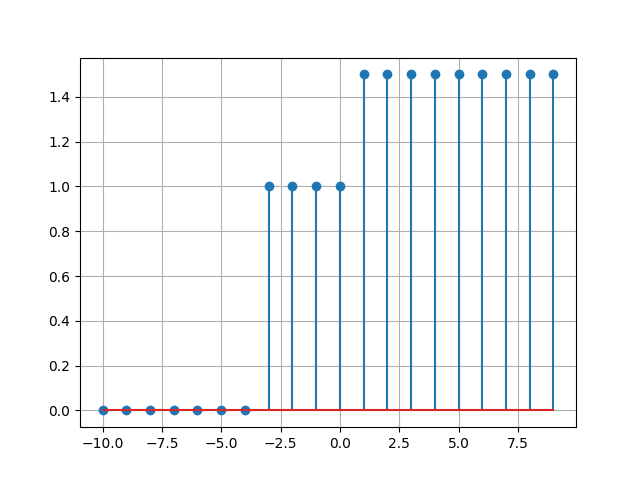
\includegraphics[width=0.5\columnwidth]{graph0.png} % Example image
  \end{center}
\item{$x[n] = -1^{n} u[-n-2]$}
  \begin{center}
    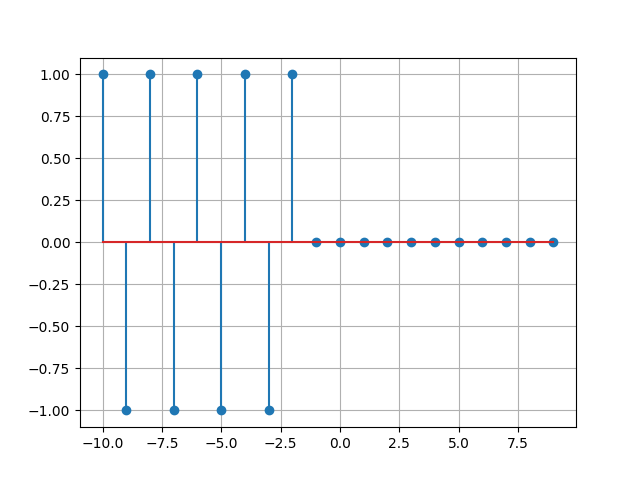
\includegraphics[width=0.5\columnwidth]{graph1.png} % Example image
  \end{center}
\item{$x[n] = \sum_{i=0}^{\infty} 4\delta[n-3k-1] $}
  \begin{center}
    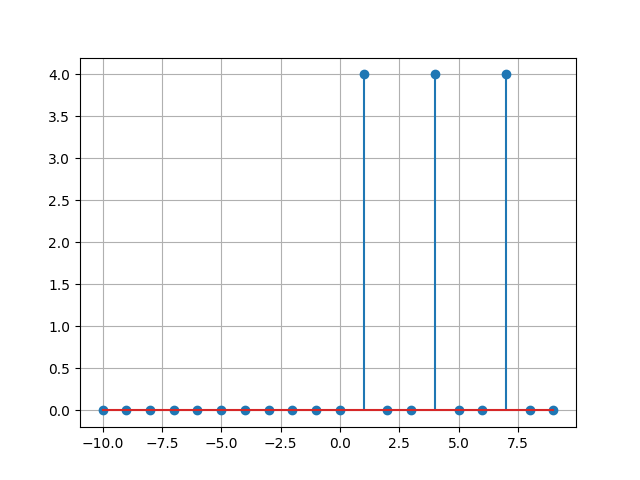
\includegraphics[width=0.5\columnwidth]{graph2.png} % Example image
  \end{center}
\end{enumerate}

\end{question}

%----------------------------------------------------------------------------------------
%	QUESTION 2
%----------------------------------------------------------------------------------------

\newpage
\begin{question}

\questiontext{Describa todas las características que sean evidentes de los siguientes sistemas}

%--------------------------------------------
\begin{enumerate}
\item{$y[n] = 3x[n-1] + 2x[n-2] + 0,75x[n+4] - 3y[n-1]$}

  \answer{
  \begin{itemize}
  \item Es un Sistema Lineal
  \item El valor de la salida depende de valores futuros de la entrada, el sistema \textbf{tiene memoria} 
  \item Debido a que la salida depende de valores futuros de la entrada el sistema \textbf{no es causal}
  \item \textbf{Sistema Inestable} por la retroalimentación
  \item Variante en el tiempo
  \end{itemize}
  }
\item{$y[n] = x[n] cos\left[ \frac{n}{2\pi}\right]$}
  \answer{
  \begin{itemize}
  \item Sistema No lineal, tiene una función periódica
  \item Invariante en el tiempo
  \item Los valores de salida n dependen solo de valores de entrada en el momento n, \textbf{sistema sin memoria}
  \item La salida no depende de valores futuros, el sistema \textbf{es causal}
  
  \end{itemize}
  }
  
\item{$y[n] = 2n^{2}x[n] + n \times x[n+1]$}

  \answer{
  \begin{itemize}
  \item \textbf{No} es un Sistema Lineal por el termino cuadratico
  \item El valor de la salida depende de valores futuros de la entrada, el sistema \textbf{tiene memoria} 
  \item Debido a que la salida depende de valores futuros de la entrada el sistema \textbf{no es causal}
  \item \textbf{Sistema Inestable}
  \item Variante en el tiempo
  \end{itemize}
  }
  
\end{enumerate}

%--------------------------------------------

\end{question}
\newpage
%----------------------------------------------------------------------------------------
%	QUESTION 3
%----------------------------------------------------------------------------------------

\begin{question}

\questiontext{Calcular la transformada Z de las 3 señales y los 3 sistemas previamente descritos.}

\begin{equation}\label{eq:uno}
  x[n]=u[n+3]+0,5u[n-1]
\end{equation}

\answer{
  \[X[z] = x[n]\cdot z^{-n}\]
  \[X[z] = \sum_{k=-3}^{-\infty} 1\cdot z^{-k} + 0,5 \sum_{k=1}^{\infty} 1 \cdot z^{-k}\]
  \[X[z] = \sum_{n=-3}^{-\infty} \left(\frac{1}{z}\right)^{n}+0,5 \sum_{n=1}^{\infty} \left(\frac{1}{z}^{n}\right)\]
  A partir de la serie geométrica:
  \[ \sum_{n=0}^{N} r^{n} = \frac{1-r^{N+1}}{1-r} \implies  \frac{\left(\frac{1}{z}\right)^{-3}-0}{1-\frac{1}{z}}+\frac{0,5\left(\frac{1}{z}\right)^{1}-0}{1-\frac{1}{z}}\]
  \[X[z]=\frac{z^3}{1-z^{-1}}+\frac{0.5\cdot z^{-1}}{1-z^{-1}}\]
  \[= \frac{z^3+0,5\cdot z^{-1}}{1-z^{-1}}\]
  expresando en positivos
  \[= \frac{z^3+0,5\cdot z^{-1}}{1-z^{-1}}\cdot\frac{z}{z}=\frac{z^4+0,5}{z-1}\]
}

\begin{equation}\label{eq:dos}
  x[n]=-1^n u[-n-2]
\end{equation}

\answer{
  \[X[z] = -1^n u[-n-2]\cdot z^{-n}\]
  \[X[z] = \sum_{n=-2}^{-\infty} -1^n\cdot z^{-n} = \sum_{n=-2}^{-\infty}-\left(\frac{1}{z}\right)^n\]
  A partir de la serie geométrica:
  \[X[z]=\frac{\left(-\frac{1}{z}\right)^{-2}-0}{1-\left(-\frac{1}{z}\right)}=\frac{\frac{1}{z^{-2}}}{1+z^{-1}}=\frac{z^2}{1+z^{-1}}\cdot \frac{z}{z}\]
  expresando en positivos
  \[X[z]= \frac{z^3}{z+1}\]
}

\newpage
\begin{equation}\label{eq:tres}
  x[n]=\sum_{k=0}^{\infty} 4\delta[n-3k-1]
\end{equation}

\answer{
  \[X[z]=4 \sum_{k=0}^{\infty} z^{-3k-1} = 4\sum_{k=0}^{\infty} \left(\frac{1}{z}\right)^{-3k-1}\]
  A partir de la serie geométrica:
  \[X[z]=4\left(\frac{\left(\frac{1}{z}\right)^{-(3\cdot0)-1}}{1-\frac{1}{z}}\right)=\frac{4z}{1-z^{-1}\cdot\frac{z}{z}}=\frac{4z^2}{z-1}\]
}

\begin{equation}\label{eq:cuatro}
  y[n]=3x[n-1]+2x[n-2]+0.75x[n+4]-3y[n-1]
\end{equation}

\answer{
  \[y[n]+3y[n-1]=3x[n-1]+2x[n-2]+0.75x[n+4]\]
  \[Y[z]+3Y[z]\cdot z^{-1} = 3X[z]\cdot z^{-1}+2X[z]\cdot z^{-2}+0.75X[z]\cdot z^4\]
  \[Y[z]\left(1+\frac{3}{z}\right)=X[z]\left(\frac{3}{z}+\frac{2}{z^{-2}}+0.75z^4\right)\]
  \[\frac{Y[z]}{X[z]}=\frac{3z^{-1}+2z^{-2}+0.75z^4}{1+3z^{-1}}\cdot \frac{z}{z}=\frac{3+2z+0.75z^5}{z+3}\]
}

\begin{equation}\label{eq:cinco}
  y[n]=x[n] cos\left[\frac{n}{2\pi}\right]
\end{equation}

\answer{
  \[Y[z]=X[z] z^0 \cdot \frac{z^2-z\cdot cos\left[\frac{n}{2\pi}\right]}{z^2-2z(cos\left[\frac{n}{2\pi}\right])+1}\]
  \[\frac{Y[z]}{X[z]}=\frac{z^2-z\cdot cos\left[\frac{n}{2\pi}\right]}{z^2-2z(cos\left[\frac{n}{2\pi}\right])+1}\]
}

\begin{equation}\label{eq:seis}
  y[n]=2n^2\cdot x[n] + n\cdot x[n+1]
\end{equation}

\answer{
  \[Y[z]=2n^2 X[z] z^{-0} + nX[z]z^1 = X[z](2n^2+zn)\]
  \[\frac{Y[z]}{X[z]}=2n^2+zn\]
}

\end{question}

%----------------------------------------------------------------------------------------

%\assignmentSection{Bonus Questions}

%----------------------------------------------------------------------------------------
%	QUESTION 4
%----------------------------------------------------------------------------------------
\newpage
\begin{question}

\questiontext{Describa que es una eigenfunción en términos de señales y sistemas.}

\answer{Lorem ipsum dolor sit amet, consectetur adipiscing elit. Praesent porttitor arcu luctus, imperdiet urna iaculis, mattis eros. Pellentesque iaculis odio vel nisl ullamcorper, nec faucibus ipsum molestie. Sed dictum nisl non aliquet porttitor. Etiam vulputate arcu dignissim, finibus sem et, viverra nisl. Aenean luctus congue massa, ut laoreet metus ornare in. Nunc fermentum nisi imperdiet lectus tincidunt vestibulum at ac elit. Nulla mattis nisl eu malesuada suscipit.}

\end{question}

\begin{question}

\questiontext{Describa las características particulares de la transformada de Laplace.}
\answer{Lorem ipsum dolor sit amet, consectetur adipiscing elit. Praesent porttitor arcu luctus, imperdiet urna iaculis, mattis eros. Pellentesque iaculis odio vel nisl ullamcorper, nec faucibus ipsum molestie. Sed dictum nisl non aliquet porttitor. Etiam vulputate arcu dignissim, finibus sem et, viverra nisl. Aenean luctus congue massa, ut laoreet metus ornare in. Nunc fermentum nisi imperdiet lectus tincidunt vestibulum at ac elit. Nulla mattis nisl eu malesuada suscipit.}
\end{question}
\newpage
\begin{question}

  \questiontext{Realice un programa, en cualquier lenguaje que prefiera, que ejecute las siguientes tareas.}
  
  \begin{itemize}
  \item{Recibe como entrada en texto plano la descripción de una señal y de un sistema, discretos ambos.}
  \item{Dibuja la señal y la respuesta al impulso del sistema.}
  \item{Ejecuta la convolución entre ambas entradas y dibujar la señal resultante.}
  \end{itemize}

  \lstinputlisting[
	caption=Luftballons Perl Script, % Caption above the listing
	label=lst:luftballons, % Label for referencing this listing
	language=Perl, % Use Perl functions/syntax highlighting
	frame=single, % Frame around the code listing
	showstringspaces=false, % Don't put marks in string spaces
	numbers=left, % Line numbers on left
	numberstyle=\tiny, % Line numbers styling
	]{luftballons.pl}

  \begin{subquestion}{How many luftballons will be output by the Listing \ref{lst:luftballons} above?} % Subquestion within question

\answer{99 luftballons.}

\end{subquestion}

  
%--------------------------------------------



%--------------------------------------------

\begin{subquestion}{Identify the regular expression in Listing \ref{lst:luftballons} and explain how it relates to the anti-war sentiments found in the rest of the script.} % Subquestion within question

\answer{Lorem ipsum dolor sit amet, consectetur adipiscing elit. Praesent porttitor arcu luctus, imperdiet urna iaculis, mattis eros. Pellentesque iaculis odio vel nisl ullamcorper, nec faucibus ipsum molestie. Sed dictum nisl non aliquet porttitor. Etiam vulputate arcu dignissim, finibus sem et, viverra nisl. Aenean luctus congue massa, ut laoreet metus ornare in. Nunc fermentum nisi imperdiet lectus tincidunt vestibulum at ac elit. Nulla mattis nisl eu malesuada suscipit.}

\end{subquestion}
  
\end{question}

\end{document}
